% Systémy barev v počítačové grafice, nelinearita grafického výstupu (gamma korekce), kompozice rastrových obrazů (alfa kanál), HDR.
\section{Systémy barev v PG}
\begin{itemize}
    \item Základem barevného prostoru je \textbf{barevný model}, který nám dává abstraktní matematický popis, jak lze barvy vyjádřit pomocí n-tic čísel, nejčastěji trojic.
    \item Mezi nejznámější barevné modely v dnešní době patří \textbf{RGB model}.
    \item Model RGB pracuje se třemi základními barvami: \textbf{červenou, zelenou} a \textbf{modrou}, z nichž se odvíjí i jeho název.
    \item Tyto barvy byly zvoleny na základně toho, jak \textbf{čípky v lidském oku} vnímají jednotlivé záření.
    \item Zároveň je RGB \textbf{aditivní barevný model}, což znamená, že se jednotlivé barevné složky \textbf{míchají} (nové barvy získáváme přidáváním větší intenzity jednotlivých složek) a výsledkem jsou další barevné odstíny, případně vyšší intenzita barvy.
    \item Když k tomuto modelu definujeme, jak mají být tyto n-tice interpretovány, dostáváme \textbf{barevný prostor} -- je předem definovaná množina barev, kterou je schopno určité zařízení snímat, zobrazit nebo reprodukovat.
    \item Barevný prostor je tedy \textbf{definován rozsahem barev}, které dokáže zobrazit.
    \item Tomuto rozsahu se také říká \textbf{gamut}. Ten se zpravidla zobrazuje jako oblast v CIE 1931 chromatickém diagramu
\end{itemize}
\begin{figure}[H]
    \centering
    \includegraphics[width=0.3\textwidth]{assets/1_rgb_gamut}
\end{figure}
\subsection{RGB}
\begin{itemize}
    \item Nejrozšířenější barevný prostor postavený na RGB barevném modelu je \textbf{sRGB} - standardní RGB.
    \item Jeho určení je pro zobrazování \textbf{na monitorech} nebo \textbf{kódování barev} na internetu.
    \item Pro všechny tři barevné složky má definované barvy v \textbf{chromatickém diagramu}, které vymezují jeho gamut.
    \item Každá barva, kterou tento prostor zobrazuje, je dána zastoupením jednotlivých barevných složek, buďto relativně (hodnoty jsou v rozmezí 0 - 1) nebo absolutně (konkrétní \uv{bitové} hodnoty, zpravidla 0 - 255, 24-bitů).
    \item RGB je možné zobrazit jako krychli.
    \item Často se přidává \textbf{Alpha kanál} pro průhlednost - \textbf{RGBA} (32-bitů).
          \begin{figure}[H]
              \centering
              \includegraphics[width=0.6\textwidth]{assets/1_rgb_gamut_krychle}
          \end{figure}
\end{itemize}

\subsection{HSV a HSL}
\begin{itemize}
    \item \textbf{Hue, Saturation, Value/Lightness} - barevný model, který nejvíce odpovídá lidskému vnímání barev.
    \item Barvy popisuje pomocí 3 hodnot, které však samy barvy nereprezentují:
          \begin{itemize}
              \item \textbf{Hue} - \textbf{barevný tón}, převládající. Neboli \textbf{odstín} - barva \textbf{odražená} nebo \textbf{procházející} objektem. Měří se jako poloha na standardním barevném kole (\ang{0} až \ang{360}). Obecně se odstín označuje názvem barvy. \ang{0} - červená, \ang{120} - zelená, \ang{240} - modrá.
              \item \textbf{Saturation} - \textbf{sytost} barvy, příměs jiné barvy. Někdy též chroma, síla nebo čistota barvy, představuje množství šedi v poměru k odstínu, měří se v procentech od 0\% (šedá) do 100\% (plně sytá barva). Na barevném kole vzrůstá sytost od středu k okrajům.
              \item \textbf{Value} - \textbf{hodnota jasu}, množství bílého světla. Relativní světlost nebo tmavost barvy. Jas vyjadřuje \textbf{kolik světla barva odráží}, dalo by se také říct přidávání černé do základní barvy.
          \end{itemize}
    \item Nejčastěji se tato reprezentace (popř. \textbf{HSL}) používají v grafických nástrojích jako komponenty pro výběr barvy, protože je mnohem intuitivnější než RGB.
    \item Vyberu si odstín, jak má být sytý a jasný a hotovo. Není třeba řešit jak smíchat 3 barevné složky, abych dostal to co chci.
    \item Dále se využívá často v případě detekce objektů, kdy hodnota HUE (odstín), je nezávislý na osvětlení scény. Problém však nastává u bílých a černých objektů (kdy HUE může být různé), ty lze na základě value a staturation mapovat do podobných barev (žlutá a černá).
    \item Mimo níže uvedené zobrazení \textbf{válcem}, lze také zobrazit \textbf{kuželem} a
          \begin{figure}[H]
              \centering
              \includegraphics[width=0.9\textwidth]{assets/1_hsv_hsl}
          \end{figure}
\end{itemize}

\subsection{CMY a CMYK}
\begin{itemize}
    \item Substraktivní barevné systémy (barvy se ,,\textbf{odečítají}'' od bílé, přidáváním jednotlivých složek až po černou), \textbf{C}yan, \textbf{M}agenta, \textbf{Y}ellow a \textbf{K}ey (Blac\textbf{K}).
    \item Používá se \textbf{pro tisk}.
    \item Černá se přidala, protože smíchání CMY nedává plně černou barvu, navíc je černý inkoust levnější než barevný.
    \item Nevýhodou je, že \textbf{nedokáže správně zobrazit} sytě červenou, zelenou a modrou.
    \item Při tisku to však není poznat.
    \item Před tiskem se RGB obraz převádí do CMYK.
    \item To provádí buďto ovladač tiskárny nebo RIP (Raster Image Processor - u profi tiskáren).
    \item RGB se používá pro aktivní zdroje světla, CMYK jsou \textbf{pasivní} (světlo pouze \textbf{odrážejí}), proto nedokáží udělat tak jasné odstíny.
\end{itemize}
\begin{figure}[H]
    \centering
    \includegraphics[width=0.6\textwidth]{assets/1_cmyk}
\end{figure}

\subsection{YCbCr}
\begin{itemize}
    \item Barva je reprezentována \textbf{jasovou složkou} Y a modrou a červenou \textbf{chrominanční} komponentou.
    \item Není to absolutní barevný model, jedná se o \textbf{způsob kódování RGB} informací.
    \item Využívá se nejčastěji u videa a barevných obrázků, kde je využito faktu, že \textbf{lidské oko nejvíce vnímá jas}, který je reprezentovaný složkou Y. Barvy už tak důležité nejsou a proto se můžou například více \textbf{komprimovat} bez výraznější ztráty kvality obrazu (JPEG).
    \item Jasová složka je kódována v intervalu $\langle0, 1\rangle$ a chrominanční složky v intervalu $\langle-0.5, 0.5\rangle$
\end{itemize}

\section{Nelinearita grafického výstupu (gamma korekce)}
První CRT monitory zobrazovaly jas nelineárně. To znamená, že dvojnásobné napětí neznamená dvojnásobný jas, křivka jasu byla zhruba exponenciální. Tento způsob zobrazení jasu přetrvává i v dnešních monitorech. Proto je potřeba upravit i zobrazované barvy. Mapování barev je potřeba provést nelineárně. Nelineární vstup v kombinaci s exponenciální křivkou jasu ve výsledku vede k k jasu, který je vnímán jako lineární. 
\begin{figure}[H]
    \centering
    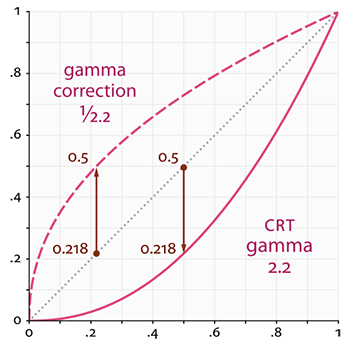
\includegraphics[width=0.3\textwidth]{assets/1_gamma_correction_gamma_curves.png}
\end{figure}
Problém nastává při práci s barvami. Pracovat s barvami je potřeba v lineárním prostoru, aby byly výsledky např. matematických operací korektní. Před zpracováním je tedy nutné převést barvu do lineárního prostou, po zpracování je potřeba před zobrazením opět převézt barvu zpět do nelineárního prostoru.

\begin{equation}
    C_{linear} = C_{sRGB}^{\text{gamma}}
\end{equation}

\begin{equation}
    C_{sRGB} = C_{linear}^{\frac{1}{\text{gamma}}}
\end{equation}

\section{Kompozice rastrových obrazů (alfa kanál)}
Alfa kanál v obrazech se používá v počítačové grafice pro průhlednost obrazů. Obrazy mohou obsahovat plnou nebo částečnou průhlednost. Plně transparentní obraz propouští veškeré barvy podkladu, částečně transparentní obraz mixuje část bravy podkladu a část vlastní barvy. Např. výsledná barva obrazu s hodnotou alfa 0.5 vytvoří mix barev tvořený z $50\%$ barvou podkladu a z $50\%$ barvou transparentního objektu. V případě překryvu více transparentních objektů je potřeba objekty setřídit dle vzdálenosti a vypočítat transparentnost postupně.   

\section{HDR}
Barvy jsou tradičně reprezentovány trojicí 8bitových hodnot v intervalu  $\langle-0, 255\rangle$. Takto popsaný obraz ale může ztrácet detaily z důvodu limitovaných možností hodnot pro rozložení barev. Přesnější metodou je ukládání jednotlivých složek jako 16 nebo 32bitových hodnot, pomocí desetiných čísel. Zde ale nastává problém s hodnotami většími než 1. Je teda nutné provést tzv. tone mapping. Proces tone mapping v zásadě převádí hodnoty do intervalu $\langle0, 1\rangle$. \par
Jednou z nejjednodušších metod je Reinhardova metoda, hodnota se vypočítá následujícím vzorcem: 
\begin{equation}
    C_{out} = \frac{C_{in}}{C_{in} + 1}    
\end{equation}
Tato metoda zachová poměrně dobře kontrast pro oblasti obrazu s nízkým jasem, oblasti obrazu s vysokým jasem jsou ale méně kontrastní. 
Pokročilejší metodou je mapování hodnot pomocí expozice, následujícím vzorcem:
\begin{equation}
    C_{out} = 1 - e^{C_{in} * \exp}
\end{equation}
Pomocí hodnoty expozice je pak možné nastavit celkové podání barev obrazu. Hodnota expozice by měla být zvolena v závislosti na aktuálním vstupu, je možné hodnotu expozice volit automaticky. 